
\documentclass[12pt]{article} 
\usepackage[utf8]{inputenc} 
\usepackage[T1]{fontenc}
\usepackage{lmodern}
\usepackage{amsmath, amssymb} 
\usepackage{hyperref}
\usepackage{geometry}
\usepackage{cite}
\usepackage[font=small,labelfont=bf]{caption}

\usepackage{graphicx}
\usepackage[
  font=small,
  labelfont=bf, 
  margin=0.5cm
]{caption}
 

\setlength{\textfloatsep}{1.2em}
\setlength{\floatsep}{1em}
\setlength{\intextsep}{1em}

\geometry{a4paper, top=3.5cm, bottom=3.5cm, left=3.5cm, right=3.5cm} 
\setlength{\parindent}{0pt}
\setlength{\parskip}{1em}

\title{Canonical Machines}
\author{Eric Hermosis \\ \texttt{eric.hermosis@gmail.com}}
\date{\today}

\begin{document}
\maketitle

\begin{abstract}
Neural networks have recently achieved unprecedented performance in emulating cognitive processes. Sequence transformer models, in particular, dominate tasks in language, speech, and vision. However, many of their mechanisms are introduced heuristically, lacking a principled theoretical foundation.

This work presents a thermodynamic model of the neuron that systematically derives common activation functions and the attention mechanism. By modeling neurons as thermodynamic systems in equilibrium in wich signal integration is modeled as a reversible process and activation as an irreversible, entropy-producing process, we link neural computation to fundamental physical principles. We extend this framework to ensembles of neurons, introducing biologically inspired excitation–inhibition and synaptic suppression mechanisms.
\end{abstract}

\section*{Introduction}

In recent years, neural networks have developed the ability to emulate certain cognitive processes with an unprecedented level of performance.

A prominent example of these architectures is sequence transformer models, known as transformers \cite{vaswani2017attention}, which have become the current paradigm for information processing in language tasks, speech recognition, and computer vision, demonstrating outstanding performance in each of these domains.

Despite their success, many of the mechanisms underlying their operation are introduced heuristically, without a theoretical framework explaining their internal dynamics. This raises the need for a conceptual approach that connects the behavior of these networks with fundamental principles of physics, allowing the interaction of their units to be interpreted as processes governed by thermodynamic and statistical laws.

In this work, we show that it is possible to develop a thermodynamic model that systematically derives the activation functions used in current architectures. This model not only explains the functioning of these mechanisms but also opens the possibility of developing new architectures and functional extensions based on physical and biological principles.

To develop this model, an artificial neuron is described as a thermodynamic system with internal energy in equilibrium with a thermal bath. Using the concept of equilibrium, the integration of signals in biological neurons \cite{dayan2001theoretical}  is modeled as a reversible process, while activation is represented as an irreversible  aforeprocess with entropy production. This framework allows for the systematic derivation of a family of widely used activation functions.
 
The same model is then used to introduce an excitation–inhibition mechanism inspired by biological neurons. Then, the attention mechanism emerges as a generalization for a model with an arbitrary number of possible responses.

To address the limitations of a single-neuron model, the concept of ensembles of models and coordinated responses is introduced, explaining within this framework the operation of classifier models and sequence transformers.

Finally, a generalization of ensembles is introduced based on the grand canonical formalism of thermodynamics. As a proof of concept, a mechanism for synaptic suppression and selective activation inspired by biological neurons is proposed.

We refer to any unit or ensemble of units whose activity follows the statistical rules of the canonical ensemble as a hermotic canonical machine.

Before addressing thementioned formalism, it is useful to first analyze the basic unit of neural networks, the neuron. This analysis allows understanding the physical origin of the model and justifying the assumptions made throughout this work.
\section*{Neurons}

Neurons are the basic units of the nervous system. Each neuron receives, processes, and transmits signals to other neurons, forming complex networks that enable everything from simple reflexes to higher cognitive processes \cite{dayan2001theoretical}.

In the brain, neurons act in a coordinated manner, integrating the information received through their dendrites and, as a result of this process, generating and communicating signals to other neurons via their axon.

The mechanism by which a neuron communicates with others is called a synapse. In every synapse, two complementary types of neurons can be distinguished: the presynaptic neuron, responsible for sending the signal, and the postsynaptic neuron, responsible for receiving and integrating it.

The dynamics of the postsynaptic neuron are determined by the signals emitted by the presynaptic neurons, whose influence is modulated by the efficacy of the synaptic connections between them.

The synaptic connections through which a neuron receives signals are called postsynaptic connections, while those through which it transmits its signal are known as presynaptic connections.

Although a biological neuron is a complex physical system, it is possible to develop a simplified computational model of it. The first formal model of a computational neuron was proposed by Warren McCulloch and Walter Pitts \cite{mcculloch1943logical} and is known as the McCulloch-Pitts neuron.

In this model, synaptic connections are represented in a binary manner (present or absent), and the neuron fires an output signal if the sum of its inputs reaches a predetermined threshold. According to the authors, this mechanism introduces a nonlinearity in the model's response.

This framework was later generalized by Rosenblatt in the perceptron model \cite{rosenblatt1958perceptron}, where synaptic connections are represented by real numbers.

The perceptron was fundamental for the development of more general approaches, such as energy-based models popularized by Yann LeCun \cite{lecun2006energy}. These models constitute a precedent in modeling neurons and neural networks as physical systems, where network behavior can be understood in terms of energetic properties, not only as heuristic models but also based on physical considerations.

Building on this precedent, a thermodynamic and statistical model for an artificial neuron is proposed below, based both on the postulates of thermodynamics formulated by B. Callen \cite{callen1985thermodynamics} and on the canonical formalism of statistical mechanics introduced by J. W. Gibbs \cite{gibbs1960statistical}.
\section*{Model}

A model is a simplified representation of a system, defined by a set of parameters that determine its behavior. A specific choice of parameters represents what we will call a configuration.

Consider the case of neurons, which are systems composed of multiple interacting physical and chemical components that integrate signals and produce responses in a nontrivial manner. Computationally describing a real neuron would be an extremely complex task and goes beyond the scope of this work. We will therefore limit ourselves to describing only idealized neuron models, which we will refer to as artificial neurons.

The simplest form of an artificial neuron is the perceptron, which can be described in terms of parameters $w^1, w^2, ..., w^d$, called synaptic weights, that allow the signals it integrates to be weighted.

We can extend the perceptron to a thermodynamic model by considering an additional parameter $U$, representing the internal energy of the neuron. With this new parameter, a perceptron configuration can be represented in terms of coordinates:

\begin{equation}
(U, w^1, ..., w^d) \in \mathbb{R}^{d+1},
\end{equation}

where the components of $\mathbf{w}$ represent the synaptic weights of the neuron, and $U$ represents an internal energy that can be considered a hidden additional parameter of the model.

To build a consistent thermodynamic framework, it is necessary to define the notion of equilibrium.
\subsection*{Equilibrium}

We say that a model is in an equilibrium configuration if we can assign it an entropy function $S$ of the parameters with the following properties:

\begin{itemize}
  \item \textbf{Extensivity}: If we consider a system composed of two models, identified as $A$ and $B$, with entropy functions $S_A$ and $S_B$, then the entropy of the combined system is:
\end{itemize}

\begin{equation}
S_{A \cup B} = S_A + S_B.
\end{equation}

\begin{itemize}
  \item \textbf{Differentiability and monotonicity}: The entropy is differentiable and monotonically increasing with respect to energy. The rate of change of entropy is always positive with increasing energy, which can be expressed as:
\end{itemize}

\begin{equation}
\frac{\partial S}{\partial U} > 0.
\end{equation}

\begin{itemize}
  \item \textbf{Maximization in the absence of constraints}: The parameter values taken in the absence of constraints are those that maximize entropy. Consequently, a system is in thermodynamic equilibrium when the following conditions are satisfied:
\end{itemize}

\begin{equation}
\delta S = 0, \qquad \delta^2 S < 0,
\end{equation}

where $\delta S$ corresponds to a virtual displacement of the entropy function. This property is known as the principle of maximum entropy.

These are the postulates proposed by B. Callen \cite{callen1985thermodynamics}, which establish the fundamental conditions for a system to be in thermodynamic equilibrium.

The second property implies that the rate of change of entropy with respect to internal energy defines strictly positive slopes, which allows the definition of an intensive parameter representing the angle of these slopes, given by:

\begin{equation}
\beta = \frac{\partial S}{\partial U}, \qquad \beta > 0,
\end{equation}

where the $\beta$ parameter can be interpreted as the reciprocal of a temperature, that is, it is possible to define a temperature $T$ for the model as:

\begin{equation}
T \equiv \frac{1}{\beta} > 0.
\end{equation}

This formalism allows us to describe a neuron as an isolated system in equilibrium in terms of its weights and a fixed internal energy. However, we are interested in modeling how it behaves under energy exchanges, so it is necessary to extend the concept of equilibrium to systems in contact with different energy sources, in particular those known as reservoirs.

Suppose the model is in equilibrium in contact with a reservoir with internal energy $U_R$ and an entropy function $S_R$. Since energy must be conserved, a virtual displacement of energy in the reservoir implies an opposite virtual displacement in the energy of the model, i.e.:

\begin{equation}
\delta U_R = -\delta U.
\end{equation}

The extensivity property of entropy tells us that the entropy of the system and the reservoir is equal to the sum of their respective entropies. Furthermore, by the principle of maximum entropy, virtual displacements in the system’s energy produce no change in the total entropy. This implies:

\begin{equation}
\delta S + \delta S_R = (\beta-\beta_R) \delta U = 0,
\end{equation}

where $\beta_R$ is the thermal parameter of the reservoir. Equilibrium is reached when the thermal parameters of the system and reservoir coincide:

This allows us to state that a model in contact with an energy reservoir is in equilibrium if both are at the same temperature. For this reason, we will refer to energy reservoirs as thermal baths.

Placing a neuron in a thermal bath allows us to describe its configurations at constant temperature. In this way, we can model energy fluctuations without breaking equilibrium. If we approximate the entropy surface to first order around a point $U_0$ associated with a configuration $(U, \mathbf{w})$, we obtain the tangent-plane equation:

\begin{equation}
S(U, \mathbf{w}) \approx S(U_0,\mathbf{w}) + \beta(U-U_0) = \Phi(\beta, \mathbf{w}) + \beta U,
\end{equation}

where $\Phi(\beta, \mathbf{w})$ is the Massieu potential, also known as free entropy, representing the intersection of the tangent plane with the origin:

\begin{equation}
\Phi(\beta, \mathbf{w}) = S(U,\mathbf{w}) - \beta U.
\end{equation}
  
This potential is a Legendre transform that allows us to describe the model in terms of the parameter $\beta$ instead of the internal energy $U$. Under this description, equilibrium is no longer characterized by a maximum of entropy $S$, but by a maximum of the Massieu potential:

\begin{equation}
\delta \Phi = 0, \qquad \delta^2 \Phi < 0
\end{equation}

Thus, the free entropy provides the necessary constraints to describe the equilibrium of a model immersed in a thermal bath, i.e., at a temperature controlled by the environment, with internal energy that can undergo variations.
\subsection*{Integration}

The signals integrated by a perceptron must carry both energy and information, because if they did not carry energy, they could not produce a physically distinguishable change in the model, and if they did not carry information, the physical change could be distinguishable but irrelevant.

If we require that the signals carry energy, their integration must produce an increase$\delta U$ in the internal energy of the model and a corresponding variation in entropy. If this variation is small, it can be expanded to first order as:

\begin{equation}
S(U+\delta U, \mathbf{w}) \approx S(U, \mathbf{w}) + \beta \delta U.
\end{equation}

Substituting this expression into the free entropy, we see that the latter remains approximately constant under small energy variations:

\begin{equation}
\Phi(\beta, \mathbf{w}) = S(U + \delta U,\mathbf{w}) - \beta (U + \delta U) \approx S(U, \mathbf{w}) - \beta U.
\end{equation}

This allows us to assert that if the energy carried by the signals is sufficiently small, the perceptron can be described as if it were in equilibrium, since the condition

\begin{equation}
\delta \Phi \approx 0
\end{equation}

is satisfied at all times. If we require that the signals carry information, then they must necessarily be associated with a probability measure, since it is uncertainty that constitutes the origin of information, according to Shannon \cite{shannon1948mathematical}.

The integration of signals precedes the perceptron’s response, known as activation. We will now show that if activation is described as an irreversible process, associated with entropy production and an energetic cost, then within an equilibrium model, an activation event can be characterized in terms of a probability. From this description, it is possible to recover a family of functions currently used to model the activation of neurons in an artificial neural network.
\subsection*{Activation}

According to Rosenblatt \cite{rosenblatt1958perceptron}, the activation of an artificial neuron results from comparing the total contribution of the integrated signals to a threshold. If this quantity exceeds the threshold, the unit produces a response, otherwise, it remains inactive.

This idea of threshold-based decision-making can be related to Maxwell’s demon \cite{maxwell1871theory}, a hypothetical entity introduced by James Clerk Maxwell to illustrate the connection between information and physical processes.

Maxwell’s demon is conceived as an entity capable of observing the microscopic state of a gas and acting selectively on a gate between two compartments, allowing only particles with higher energy to pass. As a consequence, the system would appear to evolve toward a state of lower entropy without performing work, which would seem to violate the second law of thermodynamics.

The apparent inconsistency arises from the fact that Maxwell ignored the entropy associated with the information generated by each decision. This issue is partially resolved by the mathematical theory of information developed by Claude E. Shannon \cite{shannon1948mathematical}, which quantifies the reduction of uncertainty produced by an observation or decision. The physical resolution of the problem is completed by Landauer’s principle, formulated by Rolf Landauer \cite{landauer1961irreversibility}, which states that erasing information necessarily entails an increase in entropy.

Landauer shows that the apparent decrease in entropy due to a decision is compensated by an increase in entropy elsewhere in the system. In this way, Maxwell’s demon does not violate the second law of thermodynamics. Let us now see how this idea can be applied to the activation mechanism proposed by Rosenblatt.

Suppose that the activation of a unit is a binary event with probability $p$ of occurring. According to Shannon, the information contributed by the occurrence of this event is:

\begin{equation}
I = -k \log p,
\end{equation}

where $k$ is a constant that sets the units of information. This quantity measures the reduction in uncertainty in the decision resulting from the comparison with the threshold.

On the other hand, the non-occurrence of the event also constitutes an event and, as such, contributes information.

In order to describe the neuron in a deterministic framework, we are interested in the average behavior over many realizations. The expected value of the information contributed by a model due to its activation and its complement is:

\begin{equation}
\langle I \rangle = - k \big[ p \log p + (1-p) \log(1-p) \big].
\end{equation}

Despite the negative sign, the expected value of the information is always non-negative and coincides with Shannon entropy.

\begin{figure}[h]
  \centering
  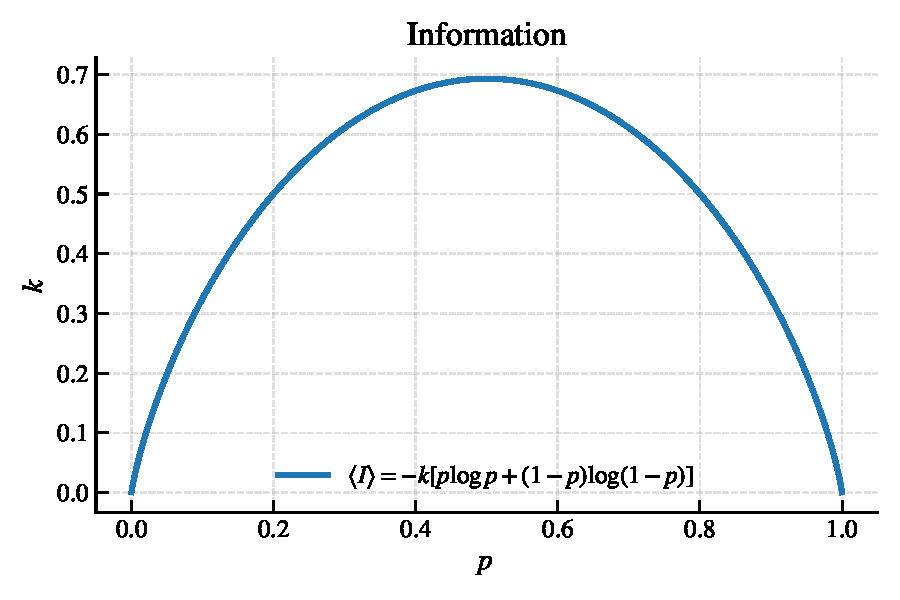
\includegraphics[width=1.0\textwidth]{assets/entropy_plot_en.pdf}
  \caption{Expected value of information $\langle I \rangle$ in units of $k$ as a function of the probability $p$ of event occurrence.}
  \label{fig:entropy_plot_en}
\end{figure}

Figure \ref{fig:entropy_plot_en} shows that the expected value of information is symmetric with respect to $p = 1/2$, where entropy reaches its maximum. This reflects that uncertainty is highest when both outcomes are equally likely. At the extremes, the expected information tends to zero, indicating that when the outcome is practically certain, the information provided is minimal.

According to Landauer, information is not an abstract entity free of physical cost, which implies a minimum production of entropy, corresponding to an increase such that:

\begin{equation}
\langle \Delta S \rangle \ge \langle I \rangle
\end{equation}

Furthermore, if the activation event is associated with an energy cost $E$, then the perceptron incurs an expected energy expenditure:

\begin{equation}
\langle E \rangle = p E
\end{equation}

This quantity can be interpreted as work performed by the model, and it provides an upper bound on the expected decrease in its internal energy such that:

\begin{equation}
\langle \Delta U \rangle \le -\langle E \rangle
\end{equation}

By taking the expected values of the changes in entropy and internal energy associated with an activation event, we impose a mean-field value to the free entropy after the ocurrence of the mentioned events:

\begin{equation}
\Phi = S + \langle \Delta S \rangle - \beta (U + \langle \Delta U\rangle).
\end{equation}

Substituting these quantities into the free entropy expression yields the inequality:

\begin{equation}
\Phi \ge S - k \big[ p \log p + (1-p) \log(1-p) \big] - \beta (U - p E)
\end{equation}

which provides a deterministic, mean-field bound for the neuron’s free entropy in terms of the activation probability $p$, the energy cost $E$, and the thermal parameter $\beta$.

Under the assumption that the model is in equilibrium, the free entropy satisfies the condition:

\begin{equation}
\delta \Phi \approx 0,
\end{equation}

in any given direction, both before and after the activation event. This implies that virtual displacements in the free entropy due to changes in the activation probability are negligible, i.e.:

\begin{equation}
\frac{\delta \Phi}{\delta p} \approx 0
\end{equation}

This translates to the approximate condition:

\begin{equation}
- k \log \left( \frac{p}{1-p} \right) + \beta E \lesssim 0
\end{equation}

The symbol $\lesssim$ indicates an approximate equality valid to first order around equilibrium, reflecting small fluctuations in the stochastic activation event.

This condition is satisfied only when the activation probability is determined by a balance between the energy cost $E$ and the thermal parameter $\beta$, giving rise to a dependency of the form:

\begin{equation}
p \gtrsim \frac{\exp\left(\frac{\beta}{k} E\right)}{1 + \exp\left(\frac{\beta}{k} E\right)} = \frac{1}{1 + \exp\left(-\frac{\beta}{k} E\right)}
\end{equation}

The resulting expression shows that the probability of an activation event is bounded by a sigmoidal relation, with equality in the ideal case.

\begin{figure}[h]
  \centering
  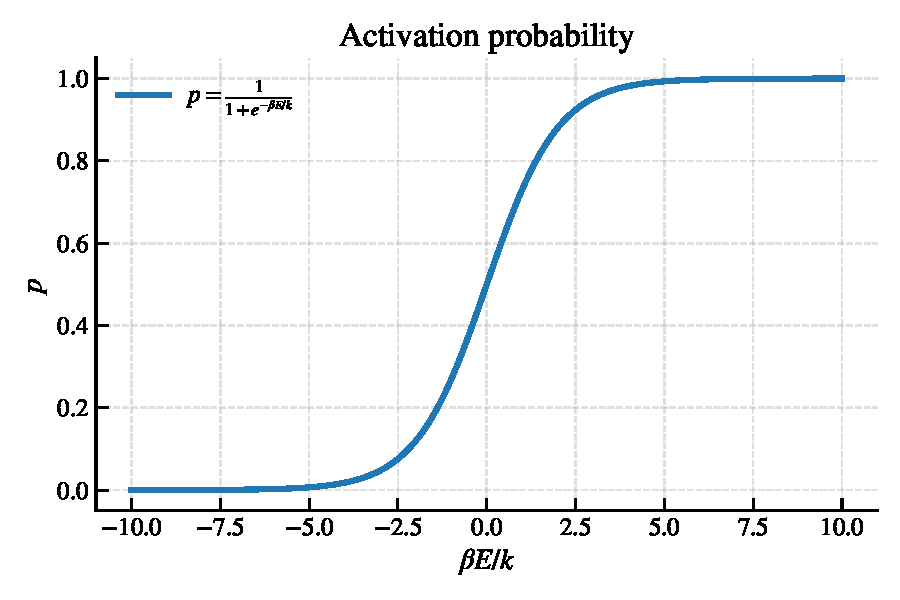
\includegraphics[width=1.0\textwidth]{assets/probability_plot_en.pdf}
  \caption{Activation probability $p$ as a function of $\beta E / k$ for an ideal neuron in thermodynamic equilibrium.}
  \label{fig:probability_plot_en}
\end{figure}

Figure \ref{fig:probability_plot_en} shows the activation probability $p$ for the ideal case. The point $\beta E / k = 1/2$ corresponds to the regime of maximum uncertainty, where both outcomes are equally probable.

In this way, the logistic regression naturally emerges from the thermodynamic equilibrium condition, and the perceptron is able to make a binary decision and generate a response based not only on its internal energy but also on its temperature as evidence.

The latter plays a role in the degree of determinism of the decision. In the low-temperature limit, thermal fluctuations are negligible and the activation probability approaches a deterministic behavior. In contrast, at high temperatures, fluctuations lead to a stochastic regime in which activation is smoothly distributed between both states, and the decision becomes inherently probabilistic.

\begin{figure}[h]
  \centering
  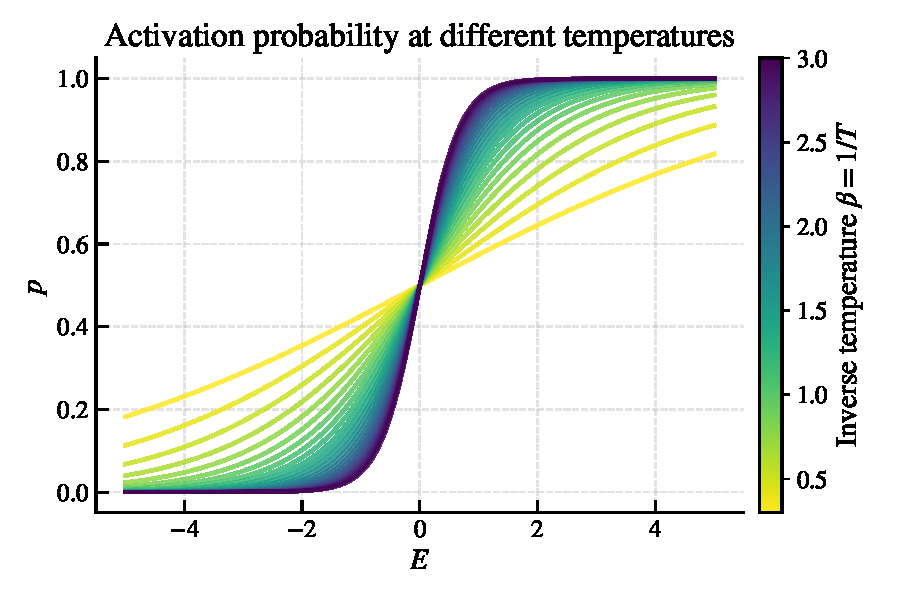
\includegraphics[width=1.0\textwidth]{assets/sigmoid_temperature_sweep_en.pdf}
  \caption{Activation probability ppp as a function of energy $E$ for different temperature values. Curves corresponding to high $\beta$ values (low temperatures) are shown in cool colors, while curves for low $\beta$ values (high temperatures) are shown in warm colors.}
  \label{fig:sigmoid_temperature_sweep_en}
\end{figure}

In figure \ref{fig:sigmoid_temperature_sweep_en}, the activation probability $p$ is plotted as a function of energy EEE for different temperatures. High $\beta$ values correspond to low temperatures, where the perceptron exhibits strongly deterministic decisions. In contrast, low $\beta$ values correspond to high temperatures, shown in warm colors (yellow and light green), and exhibit stochastic behavior, reflecting a higher degree of indecision in the response.

Based on these observations, it is convenient to define the activation potential as the dimensionless quantity:

\begin{equation}
z \equiv \frac{\beta}{k} E
\end{equation}

This potential summarizes all relevant information required to generate an activation event, as it incorporates both the energy cost associated with the event and the influence of temperature on the decision process. 

In this way, if the neuron reaches a value $z$ of the activation potential during integration, the probability of activation is determined by the sigmoid function:

\begin{equation}
\sigma(z) = \frac{1}{1+\exp(-z)} = \text{Sigmoid}(z).
\end{equation}

If the neuron’s response is proportional to the activation potential $z$, the expected value of the response defines an action potential $a$, whose value is given by the activation function known as $\text{SiLU}$ (Sigmoid Linear Unit  \cite{elfwing2018sigmoid}):

\begin{equation}
a = z \sigma(z) = \frac{z}{1+\exp(-z)} = \text{SiLU}(z).
\end{equation}

Alternatively, if the response is proportional to a value $x$ and a parameter $\gamma \propto \beta$ such that $z = \gamma x$, the action potential is described by the $\text{Swish}_{\gamma}$ family (Sigmoid-weighted Linear Unit \cite{ramachandran2017swish}):

\begin{equation}
a = \frac{x}{1+\exp(-\gamma x)} = \text{Swish}_{\gamma}(x).
\end{equation}

This family of functions interpolates between smooth and stochastic regimes for different $\gamma$ values. In the limit $\gamma \rightarrow \infty$, we obtain a deterministic action potential of the form:

\begin{equation}
\lim_{\gamma \rightarrow \infty} a =  
\begin{cases}  
0 & x < 0 \\  
x/2 & x = 0 \\  
x & x > 0  
\end{cases}
\end{equation}

Ignoring the $x = 0$ case, which has zero probability for continuous potentials in a neural network, the relevant limit reduces to the $\text{ReLU}$ (Rectified Linear Unit \cite{nair2010relu}) activation function:

\begin{equation}
a = \max(0,x) = \text{ReLU}(x).
\end{equation}

This shows that, assuming thermal equilibrium and small energy variations, neuronal activation can be described in a unified way through well-known activation functions.

\begin{figure}[h]
  \centering
  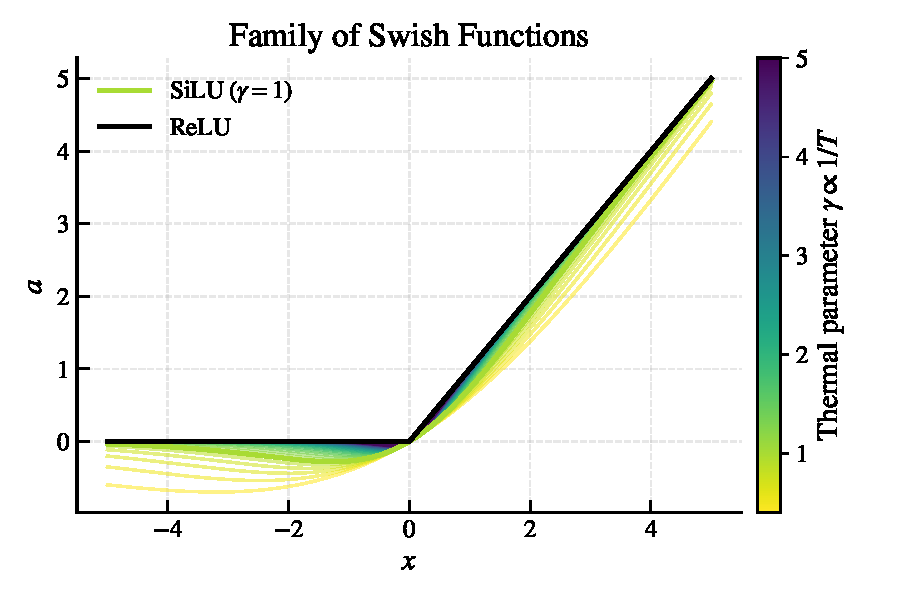
\includegraphics[width=1.0\textwidth]{assets/swish_to_relu_thermal_limit_en.pdf}
  \caption{Action potential $a$ as a function of activation potential $x$ for the Swish family at different temperatures. Curves corresponding to high $\gamma$ values are shown in cool colors (green and dark blue), while curves for low $\gamma$ values are shown in warm colors (yellow and light green). The case $\gamma = 1$ corresponds to the $\text{SiLU}$ function, and the $\text{ReLU}$ limit is indicated in black.}
  \label{fig:swish_to_relu_thermal_limit_en}
\end{figure}

The figure \ref{fig:swish_to_relu_thermal_limit_en} shows how the $\text{SiLU}$ function is recovered as a particular case of the $\text{Swish}_{\gamma}$ family. The thermal limit is reached quickly for $\gamma > 1$, producing the $\text{ReLU}$ activation function.

If the statistical model of activation is changed, different activation functions emerge. For example, modeling the system with Gaussian noise produces the $\text{GELU}$ (Gaussian Error Linear Unit \cite{hendrycks2016gelu}) activation function:

\begin{equation}
a = x F(x) = \text{GELU}(x)
\end{equation}

where $F$ is the cumulative distribution function of a standard normal. A complete description of this function is beyond the scope of this work.

Moreover, the response does not necessarily have to be proportional to the activation potential. This is the case of the recently popularized $\text{GLU}$ (Gated Linear Units \cite{dauphin2017glu}), where the expected value of the response is described as:

\begin{equation}
a = v \sigma(z) = \text{GLU}(v,z)
\end{equation}

where $v$ is a separate integrated quantity and $\sigma$ is the sigmoid function. In this way, the activation acts as a gating mechanism, deciding whether a signal passes through.

The activation functions derived here cover most of those currently used to describe neuronal activation in modern neural network architectures, including sequence-transformer models.

Within the framework developed in this work, activation functions that emerge directly from the statistical and thermodynamic principles governing canonical machines will be referred to as \textbf{hermotic activation functions}. These functions arise from the equilibrium and variational structure of the model, rather than from heuristic architectural choices.

However, some activation functions do not appear to be directly derivable from the principles presented. An example is $\text{GLU}$ variants, which have become standard in sequence transformers. Recent work \emph{GLU Variants Improve Transformer} \cite{shazeer2020glu} shows that replacing the sigmoid in $\text{GLU}$ with other activation functions can significantly improve performance. That is, it proposes an activation of the form:

\begin{equation}
a = v z \sigma(z)
\end{equation}

This approach improves results for the previously derived functions, namely $\text{SiLU}$, $\text{ReLU}$, and $\text{GELU}$. The author acknowledges that the formal reason for their success is unknown.
  
While a formal explanation of these architectures is outside the scope of this work, we make a key observation: the activation mechanism described in this section is insufficient to capture some behaviors of the model.

This limitation motivates the development of new activation models based on the variational formalism proposed here. In the next section, we propose an extension of the activation mechanism as an alternative to $\text{GLU}$ variants, derived from variational principles and inspired by biological mechanisms.
\subsection*{Excitation–Inhibition}

In a synapse, signal transmission depends both on the neurotransmitter release induced by the presynaptic action potential and on the nature of the postsynaptic receptor. In the postsynaptic neuron, depolarizations due to excitatory signals or hyperpolarizations due to inhibitory signals can occur \cite{dayan2001theoretical}.

We can model the postsynaptic response in energetic terms, associating excitatory states with decreases in internal energy due to the work performed during depolarization, and inhibitory states with increases in internal energy associated with hyperpolarization.

Now, suppose that during activation, there is not only a probability $p_+$ that the model undergoes an energy consumption $E$ but also a probability $p_-$ that the model increases its energy by the same magnitude due to a response, generating an inhibitory signal. Considering only these two responses, the expected value of the net energy change in the unit is:

\begin{equation}
\langle E \rangle = p_+ E - p_- E
\end{equation}

subject to the normalization condition $p_+ + p_- = 1$. Given these probabilities, the expected information contributed by the occurrence of this event is:

\begin{equation}
\langle I \rangle = - k (p_+ \log p_+ + p_- \log p_-)
\end{equation}

Following the same reasoning developed previously for the activation mechanism, we can approximate the internal energy and entropy variations of the model as:

\begin{equation}
\langle \Delta U \rangle \approx \langle E \rangle  
,\qquad  
\langle \Delta S \rangle \approx \langle I \rangle.
\end{equation}

Assuming thermal equilibrium again, both before and after the neuron's response, the virtual displacements of the free entropy with respect to the occurrence probabilities should be approximately zero:

\begin{equation}
\frac{\delta \Phi}{\delta p_+} \approx 0 \qquad \frac{\delta \Phi}{\delta p_-} \approx 0
\end{equation}

Next, considering a Lagrange multiplier $\lambda$, the free entropy subject to the normalization constraint, after the response, is:

\begin{equation}
\Phi \approx S - k (p_+ \log p_+ + p_- \log p_-) - \beta (U - p_+ E + p_- E) + \lambda (1 - p_+ - p_-)
\end{equation}

Using the equilibrium conditions on the probabilities, we obtain expressions for both probabilities:

\begin{equation}
\begin{aligned}  
\frac{\delta \Phi}{\delta p_+} \approx - k \log p_+ + \beta E - \lambda = 0 \  
\frac{\delta \Phi}{\delta p_-} \approx - k \log p_- - \beta E - \lambda = 0  
\end{aligned}
\end{equation}

These conditions are satisfied only for probabilities of the form:

\begin{equation}
p_+ \approx \exp(-\lambda) \exp\left(\frac{\beta}{k} E\right)
, \qquad  
p_- \approx \exp(-\lambda) \exp\left(-\frac{\beta}{k} E\right).
\end{equation}

We can now use the normalization condition to obtain an expression for the Lagrange multiplier. Summing both probabilities:

\begin{equation}
1 = \exp(-\lambda) \left(\exp\left(\frac{\beta}{k} E\right) + \exp\left(-\frac{\beta}{k} E\right)\right) = 2 \exp(-\lambda) \cosh\left(\frac{\beta}{k} E\right)
\end{equation}

Substituting, we obtain that the probabilities of a neuron generating excitatory and inhibitory responses are, respectively:

\begin{equation}
p_+ \approx \frac{\exp(\frac{\beta}{k} E)}{2 \cosh(\frac{\beta}{k} E)}, \qquad  
p_- \approx \frac{\exp(-\frac{\beta}{k} E)}{2 \cosh(\frac{\beta}{k} E)}  .
\end{equation}

This equality is imposed in the ideal case. In these expressions, a symmetry between the probabilities can be observed: changing the sign of the energy (from excitatory to inhibitory) swaps the probabilities.

\begin{figure}[h]
  \centering
  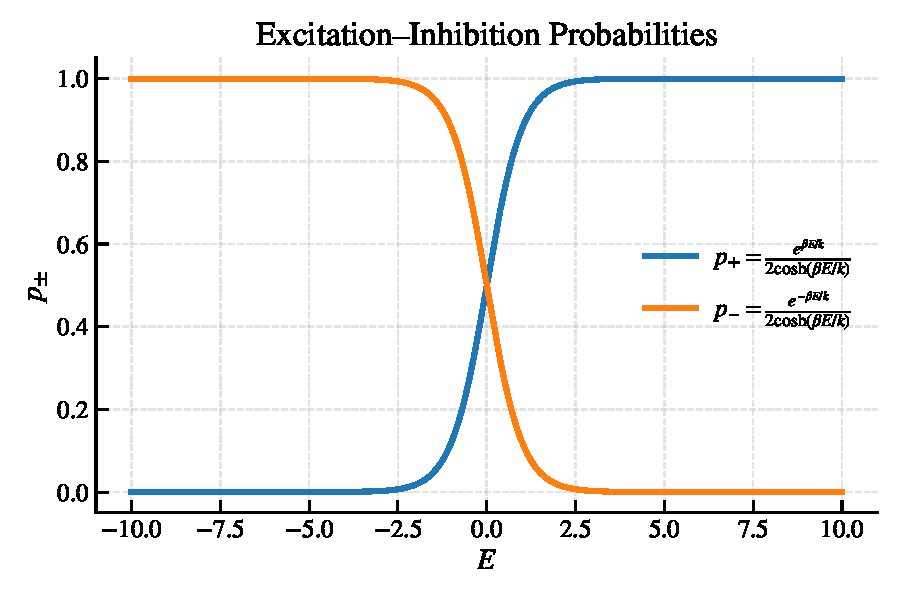
\includegraphics[width=1.0\textwidth]{assets/two_level_probabilities_en.pdf}
  \caption{Probabilities of excitatory response $p_+$ in blue and inhibitory response $p_-$ in orange as a function of the quantity $\beta E / k$.}
  \label{fig:two_level_probabilities_en}
\end{figure}
 
As illustrated in Figure \ref{fig:two_level_probabilities_en} both probabilities are symmetric under a sign change of the energy. For $E < 0$, the inhibitory response dominates ($p_- \approx 1$), while for $E > 0$, the excitatory response becomes predominant $p_+ \approx 1$. 

We observe that for negative energies, the probability of an inhibitory response is close to $1$, while the probability of an excitatory response is nearly zero. Conversely, for positive energies, excitation dominates and inhibitory responses become less likely.

The behavior of both curves is complementary, always satisfying the normalization condition. The transition between excitatory and inhibitory regimes occurs around $E = 0$, where both probabilities are equal, maximizing the uncertainty of the response.

\begin{figure}[h]
  \centering
  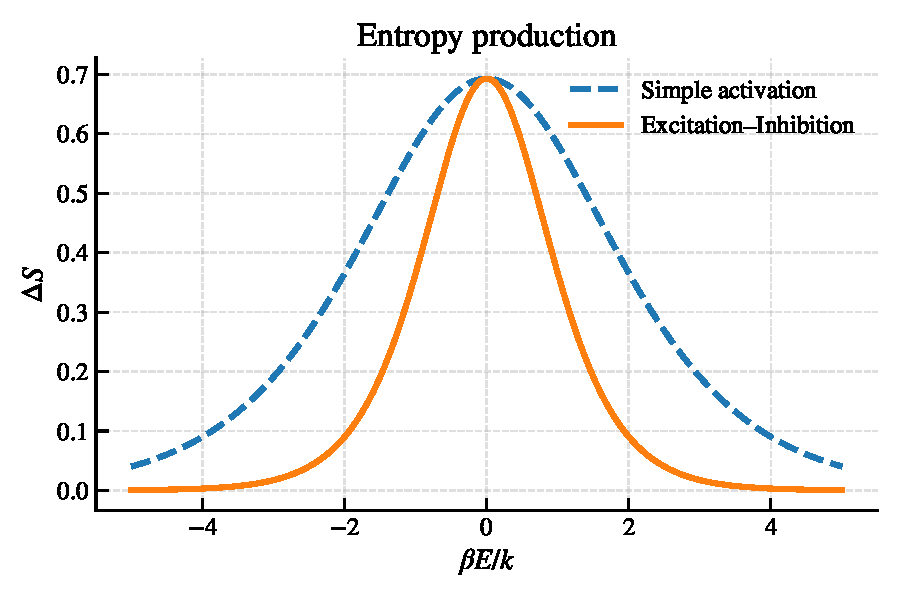
\includegraphics[width=1.0\textwidth]{assets/entropy_comparison_en.pdf}
  \caption{Entropy production associated with excitatory and inhibitory responses as a function of $\beta E / k$ (solid orange curve), compared with the case of exclusively excitatory responses (blue curve).}
  \label{fig:entropy_comparison_en}
\end{figure}

Figure \ref{fig:entropy_comparison_en} shows that the excitation–inhibition model (orange, solid) shows a sharper peak, indicating that entropy production is more sensitive to changes in energy and temperature in this regime.

Now let us see how we can model a response based on this regime. If $v$ represents an excitatory response and $-v$ an inhibitory response of equal magnitude, then the action potential generated by this model is set equal to its expected value:

\begin{equation}
a = \frac{v \exp(z) - v \exp(-z)}{2 \cosh(z)} = v \frac{\sinh(z)}{\cosh(z)} = v \tanh(z),
\end{equation}

with $z = \beta E / k$ being the previously defined activation potential. In this way, the hyperbolic tangent, a well-known and widely used activation function, also naturally emerges as an alternative for the previously mentioned $\text{GLU}$ variants.

\begin{figure}[h]
  \centering
  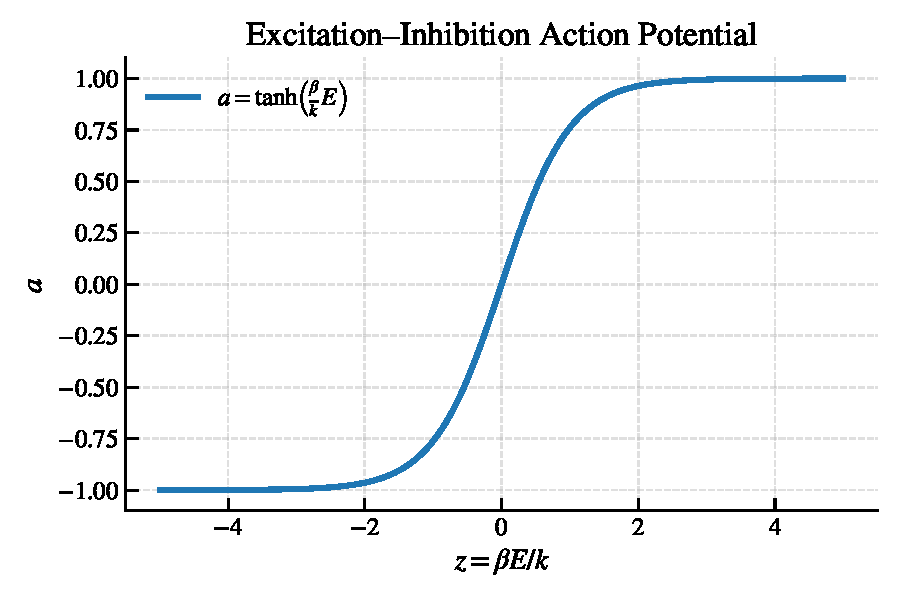
\includegraphics[width=1.0\textwidth]{assets/tanh_activation_en.pdf}
  \caption{Action potential $a = \tanh(z)$ as a function of the activation potential $z = \beta E/k$ for a constant response magnitude $v = 1$. The action potential varies continuously between $-1$ and $1$.}
  \label{fig:tanh_activation_en}
\end{figure}

In Figure \ref{fig:tanh_activation_en}, the action potential $a$ increases continuously from $-1$ to $1$. For negative $z$, inhibition dominates and $a \approx -1$; for positive $z$, excitation dominates and $a \approx 1$. Around (z=0), the expected response is zero and the uncertainty is maximal.

As with sigmoid activation functions, in an excitation–inhibition model, the determinism level of the response can also be influenced by temperature.

\begin{figure}[h]
  \centering
  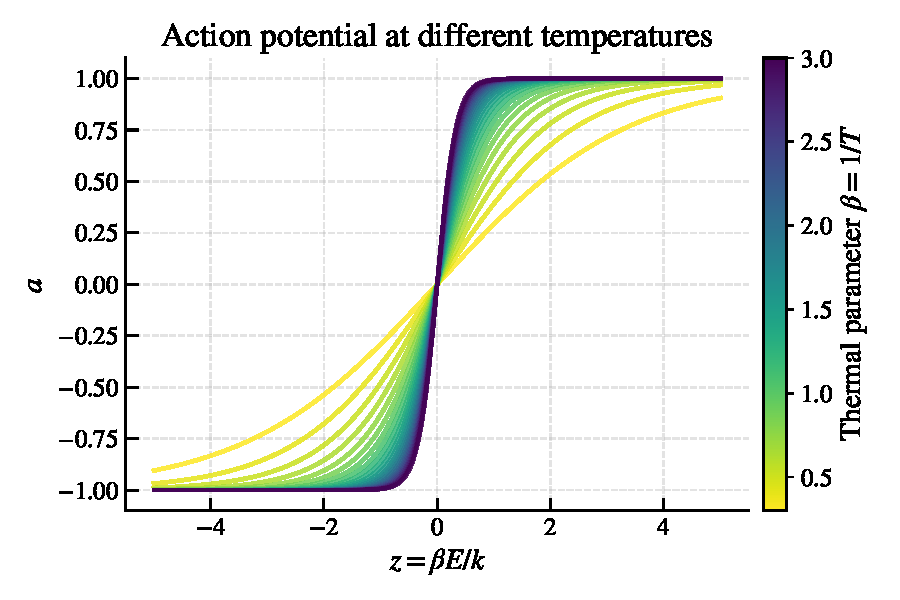
\includegraphics[width=1.0\textwidth]{assets/tanh_temperature_sweep_en.pdf}
  \caption{Action potential $a$ as a function of energy for different temperature levels in an excitation–inhibition model. Curves corresponding to low temperatures are shown in blue and violet, while high temperatures are shown in yellow and light green.}
  \label{fig:tanh_temperature_sweep_en}
\end{figure}

In Figure \ref{fig:tanh_temperature_sweep_en}, the action potential $a$ is plotted as a function of energy for different temperature levels. Curves associated with low temperatures show sharper transitions, indicating deterministic responses, while high temperatures produce smoother transitions, reflecting a more stochastic behavior.

This is just one example of how to build activation functions based on the principle of maximum entropy, and it motivates extending the formalism to discover new functions.

Next, we propose a natural generalization considering a model with arbitrary energy levels, and we will show how this idea can be used to derive the attention mechanism.
\subsection*{Attention}

So far, we have defined the energy of a state as a measure of the cost associated with a response, assigning probabilities to a small number of alternatives. However, in a more general setting, and based on ideas from physics, we can consider a unit with multiple accessible energy states, each characterized by a distinct energy level. This set of levels constitutes an energy spectrum, allowing for a more flexible modeling of a neuron that can generate different responses according to their relative cost.

Suppose a model with $l$ possible responses, each with energy costs $E_1, E_2, \dots, E_l$ and probabilities $p_1, \dots, p_l$ satisfying the normalization condition:

\begin{equation}
\sum_j p_j = 1.
\end{equation}

Under this description, the expected energy cost and the expected information contribution are:

\begin{equation}
\langle E \rangle = \sum_j p_j E_j, \qquad  
\langle I \rangle = -k \sum_j p_j \log p_j
\end{equation}

Assuming thermal equilibrium, the variational derivatives with respect to the probabilities vanish, i.e.,

\begin{equation}
\frac{\delta \Phi}{\delta p_i} \approx 0 \qquad i = 1, \dots, l
\end{equation}

We aim to maximize the free entropy subject to the normalization constraint. To do this, we introduce a Lagrange multiplier $\lambda$ so that the quantity to maximize is:

\begin{equation}
\Phi \approx S - k \sum_j p_j \log p_j - \beta \left(U - \sum_j p_j E_j \right) + \lambda \left(1 - \sum_j p_j \right),
\end{equation}

differentiating this expression, we can find the extremum conditions in terms of the probabilities, energies, and the multiplier:

\begin{equation}
-k (\log p_i + 1) + \beta E_i - \lambda \approx 0, \qquad i = 1, \dots, l,
\end{equation}

Solving for the term containing the probability, we see that it depends on the energy and the proposed multiplier $\lambda$ as a logarithm:

\begin{equation}
\log p_i \approx \frac{\beta}{k} E_i - \left(\frac{\lambda}{k} + 1\right)
\end{equation}

Taking the inverse of the logarithm on both sides and using the normalization condition, we obtain:

\begin{equation}
\sum_j p_j = \frac{1}{\exp(\frac{\lambda}{k} + 1)} \sum_j \exp\left(\frac{\beta}{k} E_j\right) = 1,
\end{equation}

from this equality, we define the partition function of the model as:

\begin{equation}
Z \equiv \exp\left(\frac{\lambda}{k} + 1\right) = \sum_j \exp\left(\frac{\beta}{k} E_j\right),
\end{equation}

then, the probability that the model incurs an energy expenditure $E_i$ is given by the distribution:

\begin{equation}
p_i = \frac{1}{Z} \exp\left(\frac{\beta}{k} E_i\right) = \frac{\exp(\frac{\beta}{k} E_i)}{\sum_j \exp(\frac{\beta}{k} E_j)}
\end{equation}

This expression formally resembles the Boltzmann distribution but differs in the sign of the exponents and its meaning, since we are not calculating the probability of the neuron reaching an energy level but rather the probability of incurring an energy expenditure.

In this way, a neuron that integrates stronger signals can generate more “aggressive” responses. Thus, states with higher energy expenditure are statistically favored, as they reduce the neuron’s internal energy more, naturally capturing the relationship between the magnitude of integration and a neuron’s propensity to activate.

Now consider a potential vector $\mathbf{z} \in \mathbb{R}^l$ whose components are the activation potentials:

\begin{equation}
z_i = \frac{\beta}{k} E_i \qquad i = 1, 2, \dots, l
\end{equation}

We can define a mass function for each coordinate of the potential, describing the probability distribution governing the model’s responses as:

\begin{equation}
\rho_i(\mathbf{z}) = \frac{\exp(z_i)}{\sum_j \exp(z_j)} = \text{Softmax}(\mathbf{z})_i.
\end{equation}

Although this result might suggest that a unit is capable of performing a classification task, since the function is the same as that used in classifiers, this is not the case, as a neuron can generate only a single signal. If $v^1, v^2, \dots, v^l$ are the possible responses, the action potential corresponds to the expected value:

\begin{equation}
a = \sum_j \rho_j(\mathbf{z}) v^j
\end{equation}

This result instead partially describes the attention mechanism used in sequence transformers, since the obtained expression is identical to self-attention if the activation potential is considered as an interaction between two signals from the same sequence, i.e., assuming that the potential coordinates are due to an interaction of the form:

\begin{equation}
z_i = \gamma \mathbf{q} \cdot \mathbf{k}_i \qquad i = 1, \dots, l,
\end{equation}

with $\gamma \in \mathbb{R}$ a scalar, $\mathbf{q}$ representing a query, and $\mathbf{k}_i$ representing one of the possible keys. Then the action potential takes the form:

\begin{equation}
a = \sum_j \text{Softmax}(\gamma \mathbf{q} \cdot \mathbf{k}_j) \cdot v^j
\end{equation}

which coincides with the self-attention mechanism expression in a one-dimensional model if the sum is identified as the inner product between the distribution and the corresponding responses.

The idea of query, key, and value was formally introduced in the context of sequence transformer models in the work \emph{“Attention Is All You Need”}, which introduced the self-attention mechanism \cite{vaswani2017attention}. A direct physical approach to these quantities is left as future work.

In any case, it is meaningless to study such models with an individual neuron, so it is necessary to introduce the concept of an ensemble, allowing the modeling not only of individual neuron responses but also the coordinated responses that emerge in layers of neurons.
\section*{Ensembles}

The success of artificial neural networks stems from the ability of neurons to work together and generate coordinated responses. This coordination allows for specialization and division of labor, a neural network can decompose a complex task into multiple simpler tasks, which can be handled by specialized units.

From a thermodynamic perspective, a set of interacting neurons can be viewed as a thermodynamic ensemble whose components exchange energy and information and produce entropy. Within this framework, coordination can be interpreted as a consequence of the extensivity of certain thermodynamic quantities associated with neurons, such as internal energy and entropy.
\subsection*{Canonical Ensemble}

Consider now an ensemble of $n$ neurons of the same dimension, which we will refer to as a layer. The extensive property of internal energy allows us to model the neuron ensemble with a single internal energy $U$, so that a configuration can be written in terms of the coordinates:

\begin{equation}
(U, \mathbf{w}_1, \ldots, \mathbf{w}_n) \in \mathbb{R} \times \mathbb{R}^{d} \times \cdots \times \mathbb{R}^d
\end{equation}

where $\mathbf{w}_i \in \mathbb{R}^d$ represents the synaptic weights of the $i$-th neuron. It is natural to group these vectors into a single matrix $\mathbf{W} \in \mathbb{R}^{n \times d}$, so that the layer’s configuration can be compactly written as:

\begin{equation}
(U, \mathbf{W}) \in \mathbb{R} \times \mathbb{R}^{n \times d}
\end{equation}

The concepts of equilibrium and entropy can be defined analogously to the case of a single neuron.

The fundamental difference between a single neuron and a layer of neurons lies in the number of responses these models can generate. While a single neuron produces only one response, a layer of $n$ neurons can produce up to $n$ different responses.

The simplest case occurs when responses are modeled as independent of each other, so that the activation dynamics of each neuron are identical to those if modeled individually. This assumption justifies the use of activation functions applied component-wise in layers of a deep network.

On the other hand, a layer of neurons can generate a joint response, whose meaning exceeds that of the individual responses of its components and may exhibit collective response modes emerging from interactions and competition among the units.
\subsubsection*{Classifiers}

If we consider that the spectrum of posible responses produced by layer of $n$ neurons is asociated with $n$ energies $E_1, E_2, \ldots, E_n$ costs, and under the hypothesis of thermal equilibrium, following the maximum entropy principle developed in previous sections, the probability $p_i \ge 0$ of the layer incurring an energy expenditure $E_i$ is, according to the previous section:

\begin{equation}
p_i \approx \frac{1}{Z} \exp\left(\frac{\beta}{k} E_i\right)  
= \frac{\exp\left(\frac{\beta}{k} E_i\right)}{\sum_j \exp\left(\frac{\beta}{k} E_j\right)}.
\end{equation}

This expression defines a statistical competition among the different collective states: those associated with higher energy potentials are more likely to be realized, while the others are more likely to be suppressed.

Given the potential vector $\mathbf{z} \in \mathbb{R}^n$, the response generated by the layer is characterized by the distribution:

\begin{equation}
\rho(\mathbf{z}) = \text{Softmax}(\mathbf{z}),
\end{equation}

which assigns to each component a probability quantifying its relative contribution to the collective state.

This shows that, unlike a single neuron, a layer of $n$ neurons can perform a classification task, as it can represent an $n$-ary categorical distribution, where each component of the response corresponds to the estimated probability of membership.
\subsubsection*{Transformers}

Another construct that can naturally be described by layers with joint responses is the attention mechanism used in sequence transformer models.

A sequence transformer model is a type of deep neural network designed to process sequential data, where each element of the sequence can interact with all others through an attention mechanism \cite{vaswani2017attention}.

We are interested in interpreting a transformer as an ensemble of neurons organized in layers, where each layer can generate joint responses depending on interactions among its units. This allows us to model the dynamics of each layer within a thermodynamic framework.

Suppose a layer of $n$ neurons, each with an energy spectrum of $l$ levels. Under this description, each neuron can generate $l$ possible responses, associated, for example, with different positions in an input sequence.

We assign to each neuron a distributed response $\mathbf{v}_i \in \mathbb{R}^l$, whose components represent the possible responses of the $i$-th neuron. It is convenient to introduce matrix notation for sequences, so that the sequence of responses can be represented as a matrix $\mathbf{V} \in \mathbb{R}^{l \times n}$, where each column corresponds to the distributed response of a neuron.

Similarly, we denote by $\mathbf{Z} \in \mathbb{R}^{l \times l}$ the matrix of activation potentials, whose elements quantify interactions between queries and keys. These potentials are imposed via the product:

\begin{equation}
\mathbf{Z} = \gamma \mathbf{Q} \cdot \mathbf{K},
\end{equation}

where $\gamma \in \mathbb{R}$ is a scaling factor, and $\mathbf{Q}, \mathbf{K}$ represent the query and key sequences, respectively, as mentioned earlier. The entries of the activation potential matrix are thus:

\begin{equation}
z^i{}_j = \gamma \mathbf{q}^i \cdot \mathbf{k}_j \qquad i,j = 1,\dots,l,
\end{equation}

where $\mathbf{q}^i$ is the $i$-th row of the query matrix $\mathbf{Q}$, $\mathbf{k}_j$ the $j$-th column of the key matrix $\mathbf{K}$, and $\cdot$ denotes an inner product in $\mathbb{R}^l$. Finally, the sequence of joint action potentials generated by the layer is:

\begin{equation}
\mathbf{A} = \text{Softmax}(\gamma \mathbf{Q} \cdot \mathbf{K}) \mathbf{V}.
\end{equation}

This corresponds to the expression used attention mechanism. The precise nature of the interactions generating the activation potential matrix $\mathbf{Z}$ is beyond the scope of this work. Recent techniques, such as Rotary Positional Embeddings (RoPE) \cite{su2021roformer}, incorporate positional information through complex rotations in the query and key space, suggesting that these signals could be conceptualized as waves in a complex space. Verifying this hypothesis is left as future work.

While the canonical ensemble adequately explains the attention mechanism when the set of interactions is fixed, it does not address how these interactions may vary dynamically according to the length of the transformed sequence. In this work, we do not analyze this aspect in detail, but we propose a new type of ensemble that extends the canonical model and allows the description of systems with a variable number of active units, thereby capturing the dynamic nature of certain attention models.
\subsection*{Grand Canonical Ensemble}

Suppose we have a layer with internal energy $U$, and we introduce a new extensive quantity $N$, which we call the occupation number, representing the number of models actively participating in inference.

If the layer is in equilibrium, we can assign it a differentiable entropy function according to the postulates. With this, we introduce the intensive parameter conjugate to the occupation number, defined as:

\begin{equation}
\alpha \equiv \frac{\partial S}{\partial N}.
\end{equation}

This parameter is related to the chemical potential in thermodynamics via the quotient:

\begin{equation}
\mu = -\frac{\alpha}{\beta},
\end{equation}

where $\beta$ is the inverse temperature. Analogous to the case of an individual model, it is natural to consider the thermodynamic potential obtained via the Legendre transform of the entropy with respect to $U$ and $N$:

\begin{equation}
\Phi(\alpha, \beta, \mathbf{W}) = S(U, \mathbf{W}, N) - \beta U + \alpha N.
\end{equation}

This potential provides an appropriate description of the system when internal energy can be exchanged with the environment and the number of actively participating models during inference can vary. The equilibrium of the ensemble is again characterized by the extremum condition:

\begin{equation}
\delta \Phi = 0, \qquad \delta^2 \Phi < 0,
\end{equation}

this time considering virtual displacements in the occupation number as well. This potential generalizes the previously derived one, as it reduces to the same equilibrium conditions for a fixed occupation number.

If the energy increases by $\delta U$ and the occupation number decreases by $\delta N$, the entropy undergoes a displacement:

\begin{equation}
S(U+\delta U, \mathbf{W}, N- \delta N) = S(U, \mathbf{W},N) +\beta \delta U - \alpha \delta N.
\end{equation}

For this configuration, the free entropy is:

\begin{equation}
\Phi(\alpha, \beta, \mathbf{W}) = S(U+\delta U, \mathbf{W}, N- \delta N) + \beta(U + \delta U) - \alpha (N-\delta N),
\end{equation}

substituting and expanding the terms, we see that this potential is conserved for small displacements of internal energy and occupation number.

In this way, the introduction of the occupation number and its conjugate parameter allows us to characterize the equilibrium of a layer when certain units are more active than others, without compromising the global stability of the ensemble.

This approach not only generalizes the case of a layer with a fixed number of units but also opens the possibility of modeling selective activation dynamics: some neurons may contribute more to the collective state while others are temporarily inactive. This idea naturally connects to phenomena observed in neuroscience, such as synaptic supression.
\subsubsection*{Suppression}

In neuroscience, synaptic elimination has been studied for decades as a central component of nervous system development, associated with circuit refinement. The loss of connections is not interpreted as a failure, but rather as a necessary condition for robust functional patterns to emerge \cite{huttenlocher1979synaptic}.

An example of this mechanism is synaptic pruning, described as a process that refines circuits by selecting the most functional synapses and eliminating the least used ones. Studies such as those by Huttenlocher showed that, in the human brain, synaptic density initially exceeds system requirements and then decreases, ensuring that only the most relevant connections persist \cite{huttenlocher1979synaptic}.

This biological principle inspired techniques in artificial neural networks, such as Optimal Brain Damage \cite{lecun1989optimal} and later Optimal Brain Surgeon \cite{hassibi1993second}, in which less important weights are eliminated to reduce network complexity without compromising performance. Today, synaptic pruning is a standard method for optimizing and simplifying deep neural networks.

Another elimination mechanism is synaptic suppression, which differs from pruning in that it corresponds to the dynamic inactivation of certain synapses without necessarily removing them permanently. This process prioritizes more relevant signals and suppresses less necessary transmission.

Attempts have been made to introduce synaptic suppression in artificial networks, for instance through methods like DropConnect \cite{wan2013regularization}, which stochastically drop weights during training. However, these methods primarily serve as regularization techniques and are disabled during inference, not considering the statistical nature of the network.

We now propose a structural synaptic suppression mechanism based on the grand canonical ensemble formalism, which not only aims to improve model training but also remains effective during inference.

Consider an individual neuron immersed in a thermal bath and subject to a chemical potential. Suppose the postsynaptic connection is suppressed with probability $q = 1-p$, independent of the neuron’s activation probability. The information contributed by the suppression is:

\begin{equation}
\langle I \rangle = -k \big( p \log p + (1-p) \log(1-p) \big),
\end{equation}

analogous to the entropy of a binary activation, reflecting the information content of the decision to suppress or maintain the connection.

Consistently with our thermodynamic framework, the expected energy cost after generating an action potential, accounting for suppression, is:

\begin{equation}
\langle E \rangle = p E.
\end{equation}

For an ensemble composed of a single model, the occupation number is simply $1$. Then, suppression reduces the occupation number by the expected amount:

\begin{equation}
\langle n \rangle = 1-p.
\end{equation}

Incorporating these quantities into the ensemble’s free entropy, accounting both for the entropy contribution from the suppression decision and the changes in internal energy and occupation number, we obtain:

\begin{equation}
\Phi \approx S - k \big[ p \log p + (1-p) \log(1-p) \big] - \beta (U-p E) + \alpha p.
\end{equation}

Using the equilibrium condition $\delta \Phi \approx 0$, which maximizes free entropy, we obtain the approximate expression:

\begin{equation}
\frac{\delta \Phi}{\delta p} \approx -k \log \left(\frac{p}{1-p}\right) + \beta E + \alpha \approx 0.
\end{equation}

This holds only when the probability that the unit is not suppressed takes the form:

\begin{equation}
p \approx \frac{1}{1+\exp(-\frac{\beta}{k}E-\frac{\alpha}{k})} = \frac{1}{1+ \exp(-\frac{\beta}{k}(E - \mu))}.
\end{equation}

This shows that the chemical potential $\mu$ acts as a threshold, suppressing neuronal activation depending on its potential.

\begin{figure}[h]
  \centering
  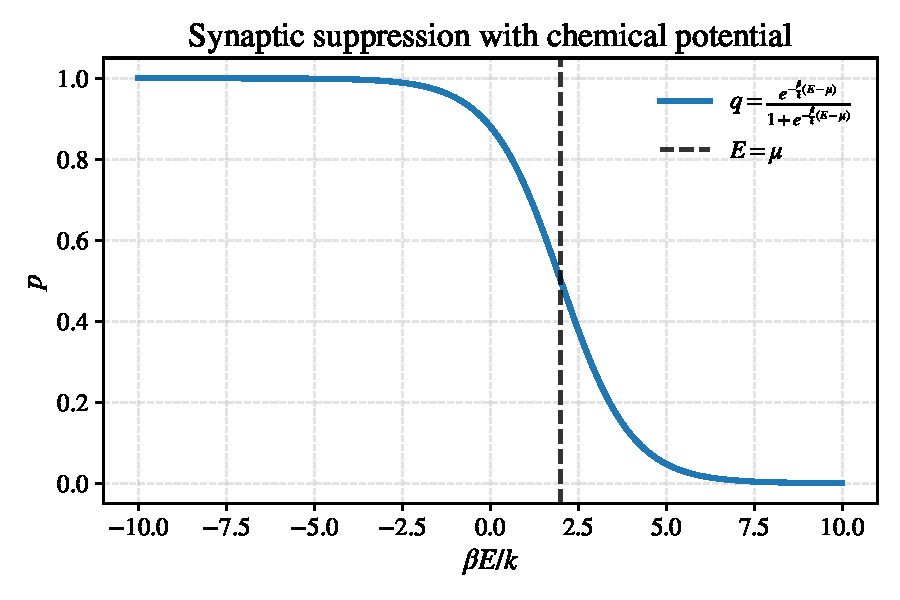
\includegraphics[width=1.0\textwidth]{assets/synaptic_suppression_threshold_en.pdf}
  \caption{Probability of supression as a function of energy $E$ and chemical potential $\mu$ (dashed vertical line).}
  \label{fig:synaptic_suppression_threshold_en}
\end{figure}

Figure \ref{fig:synaptic_suppression_threshold_en} shows that for $E<\mu$ the supression probability approaches $1$, whereas for $E>\mu$ it decreases quickly, reflecting suppression of less active connections and prioritization of energetically relevant signals.
 
If $z$ is the activation potential and $\theta = k \alpha$ is a reparameterization of the chemical parameter, the probability of a neuron’s postsynaptic connection not being suppressed can be represented by the sigmoidal function:

\begin{equation}
\sigma(z-\theta) = \frac{1}{1+ \exp(-z + \theta)}.
\end{equation}

Changes in the chemical parameter modulate the contribution of each neuron to the ensemble’s collective activity:

\begin{itemize}
  \item If $z \gg \theta$, the connection is very unlikely to be suppressed ($\sigma(z-\theta) \approx 1$).
\end{itemize}
    
\begin{itemize}
  \item If $z \ll \theta$, suppression is almost certain ($\sigma(z-\theta) \approx 0$).
\end{itemize}
    

Thus, the chemical potential regulates the neuron’s effective activation. Increasing $\theta$ shifts the sigmoid to the right, increasing suppression probability for the same potential, while decreasing $\theta$ has the opposite effect.

\begin{figure}[h]
  \centering
  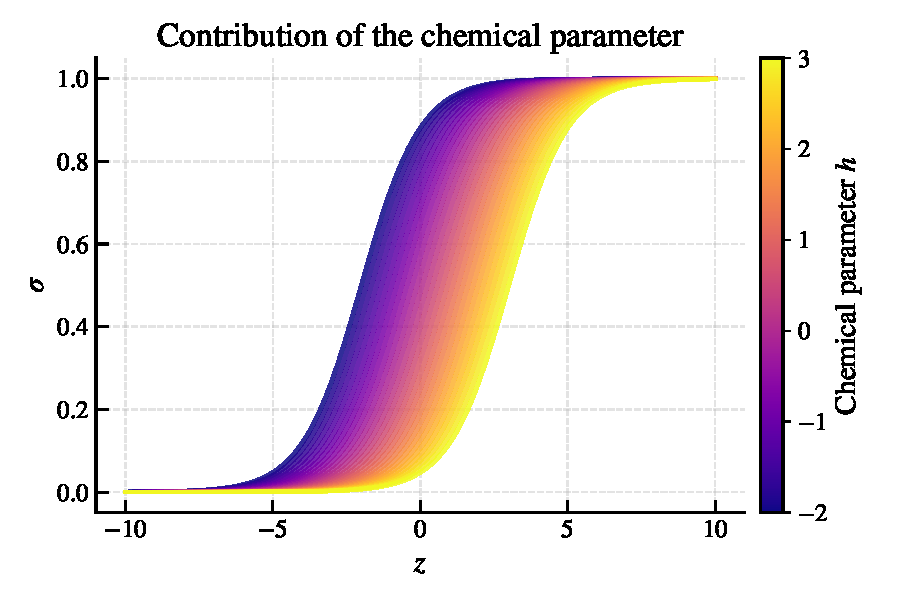
\includegraphics[width=1.0\textwidth]{assets/synaptic_suppression_property_en.pdf}
  \caption{Probability of postsynaptic connection survival $\sigma(z-\theta)$ as a function of activation potential $z$ for different values of chemical parameter $\theta$ shown in different colors.}
  \label{fig:synaptic_suppression_property_en}
\end{figure}

Figure \ref{fig:synaptic_suppression_property_en} shows that increasing $\theta$ shifts the sigmoid rightward, increasing suppression probability for a given $z$, while decreasing $h$ shifts it leftward.

Therefore, if a neuron has an activation function $f$ asociated with response $v$, the action potential considering suppression is:

\begin{equation}
a = \sigma(z-\theta) f(z) v.
\end{equation}

For instance, if $f = \tanh$ and $v=1$, the chemical potential suppresses inhibitory synapses, allowing excitatory synapses to dominate.

\begin{figure}[h]
  \centering
  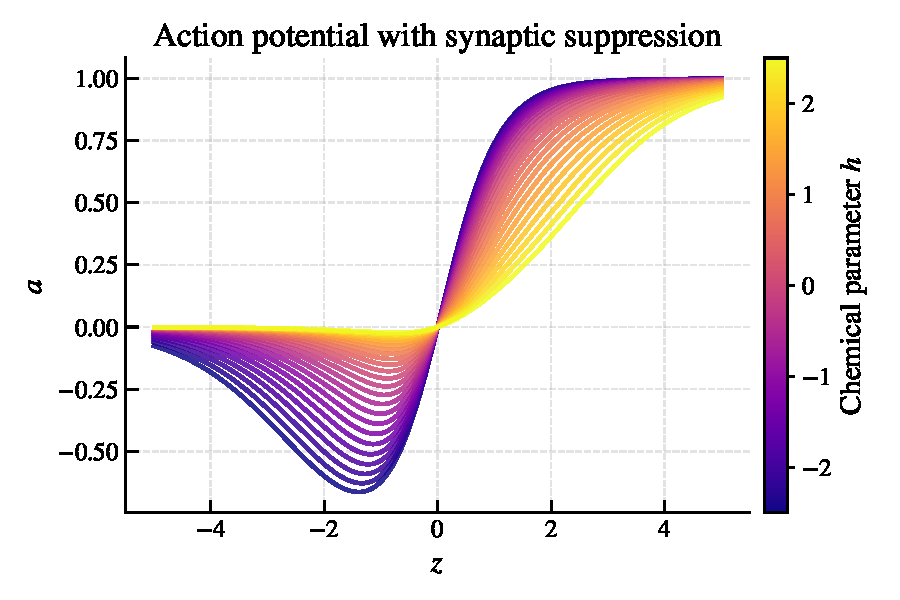
\includegraphics[width=1.0\textwidth]{assets/suppressed_tanh_activation_sweep_en.pdf}
  \caption{Resulting action potential $a=\sigma(z-\theta)\tanh(z)$ as a function of activation potential $z$ for different chemical parameter values $\theta$. This figure combines the excitation-inhibition mechanism with synaptic suppression.}
  \label{fig:suppressed_tanh_activation_sweep_en}
\end{figure}

The figure \ref{fig:suppressed_tanh_activation_sweep_en} shows the following effects of synapse supression:

\begin{itemize}
  \item For $\theta \ll 0$ suppression is minimal, and the action potential follows the original $\tanh$ almost entirely.
\end{itemize}
    
\begin{itemize}
  \item For intermediate $\theta$ values, inhibitory signals are partially suppressed, generating asymmetry in excitation-inhibition.
\end{itemize}
    
\begin{itemize}
  \item For $\theta \gg 0$ suppression is strong: even moderately activated neurons are silenced, and only neurons with $z \gg \theta$ generate significant action potentials.
\end{itemize}
    

This demonstrates how introducing a synaptic suppression mechanism extends known response mechanisms.

This idea can also be applied to the attention mechanism. To capture this dynamic within the grand canonical ensemble framework, the partition function must be modified to incorporate suppression, reflecting that some neurons contribute less or not at all to the collective state:

\begin{equation}
Z = \sum_j \sigma(z_j-h) \exp(z_j),
\end{equation}

where each term weights the neuron’s contribution by its probability of not being suppressed and its relative energy. Neurons with $z_j \ll \theta$ have little influence on the ensemble dynamics, whereas those with $z_j \gg \theta$ dominate the response.

From this partition function, we define the probability distribution governing attention:

\begin{equation}
\rho(\mathbf{z}, \theta)_i =\frac{ \sigma(z_i- \theta) \exp(z_i)}{\sum_j \sigma(z_j-\theta) \exp(z_j)}.
\end{equation}

In the limit $\theta \to -\infty$, the sigmoid tends to 1 for all neurons, eliminating suppression effects. This shows that a model considering synaptic suppression via a chemical potential is at least as expressive as a model without suppression.

Thus, we have introduced a synaptic suppression mechanism derived from the grand canonical ensemble formalism, showing how the chemical potential acts as a threshold that regulates neuron contribution both at the individual activation level and in collective mechanisms such as attention.

While this framework provides a consistent thermodynamic interpretation, it remains to be evaluated empirically. In particular, the effects of excitation-inhibition and synaptic suppression on model behavior during training and inference need to be tested.
\section*{Conclusion}

In this work, we established a thermodynamic and statistical framework to describe artificial neurons, in which signal integration and response generation are interpreted as processes consistent with the laws of thermodynamics.

We showed that, by considering the neuron in equilibrium with a thermal bath and neuronal activation as an irreversible process accompanied by entropy production, it is possible to naturally derive the probability of activation as a function of its internal energy and the thermal parameter of the environment.

This approach explains widely used activation functions in neural networks, such as $\text{ReLU}$, $\text{SiLU}$, and variants of $\text{Swish}$, showing how temperature regulates the stochastic or deterministic character of the response. Extending the model to excitation–inhibition scenarios revealed how neurons can generate complementary responses and allowed the $\tanh$ function to emerge as a natural activation function. 

Furthermore, by considering a spectrum of possible responses, the attention mechanism in neural networks was described, where the probability of generating each response depends on the corresponding activation potential.

Within this framework, the neuron can be interpreted as the simplest hermotic canonical machine, that is, a computational unit whose response follows the statistical structure of a canonical ensemble.

The individual description of the neuron was then extended to ensembles of neurons, interpreting layers of neural networks as thermodynamic systems whose components exchange information and produce entropy. Coordination among units enables the generation of joint responses that exceed the sum of individual responses, explaining the ability of layers to represent categorical distributions through $\text{Softmax}$ and to perform classification and attention tasks.

The generalization to the grand canonical ensemble introduced the occupation number and its conjugate parameter associated with the thermodynamic chemical potential. As a proof of concept, this formalism was shown to model phenomena of selective activation and synaptic suppression, using a chemical parameter as a threshold regulating the contribution of each neuron to the collective state of a layer.

This approach suggests new principles for the design and optimization of deep neural networks, connecting theory with functional mechanisms observed in neuroscience and providing tools to model complex dynamics of selective activation and cooperation between units.
\newpage
\bibliographystyle{unsrt}
\bibliography{references}
\end{document}
